\documentclass{article}
\usepackage[screen,left=0.5in,textwidth=5in,marginparwidth=3in]{geometry}
\usepackage{alltt,fancyvrb,framed,xcolor,marginnote}
\usepackage[utf8]{inputenc}
\usepackage{listings}
\usepackage{graphicx}
\colorlet{shadecolor}{yellow!30}
\lstset{
belowcaptionskip=1\baselineskip,
xleftmargin=\parindent,
breaklines=true, %% Wrap long lines
language=C++,
escapeinside={/*}{*/},
escapebegin=\begin{shaded}\obeylines\obeyspaces,
escapeend=\end{shaded},
showstringspaces=false,
basicstyle=\small\ttfamily,
commentstyle=\itshape\color{gray},
stringstyle=\color{black},
keywordstyle=\bfseries\color{green},
identifierstyle=\color{blue},
%numbers=left,
}
\begin{document}



\newpage\section*{Specification}
\begin{verbatim}
The program will prompt you for a file name. It will then display each sentence on a new line.
\end{verbatim}


\newpage\section*{Analysis}
\begin{description}
  \item[Input] There is no input required by the program.
  \item[Process] The program will prompt the user for a file name. The content of that will then be iterated through. if the character is a punctuation character and is not in the middle of quotes then it will put a newline after it.
  \item[Output] Displays every sentence from the file on a new line.
\end{description}

\newpage\section*{Design}
\begin{itemize}
	\item lab.cpp : Will ask for user input for file name. The content of the will then pass it to searchPunc()
	\item searchPunc.cpp : Will iterate through each character, if the character is a punctuation character and is not in the middle of quotes then it will put a new line after it.
\end{itemize}

\newpage\section*{Implementation}

\lstinputlisting{src/lab.h}\newpage

\lstinputlisting{src/lab.cpp}\newpage

\lstinputlisting{src/searchPunc.cpp}\newpage

\newpage\section*{Testing}
\subsection*{Testcase 1}
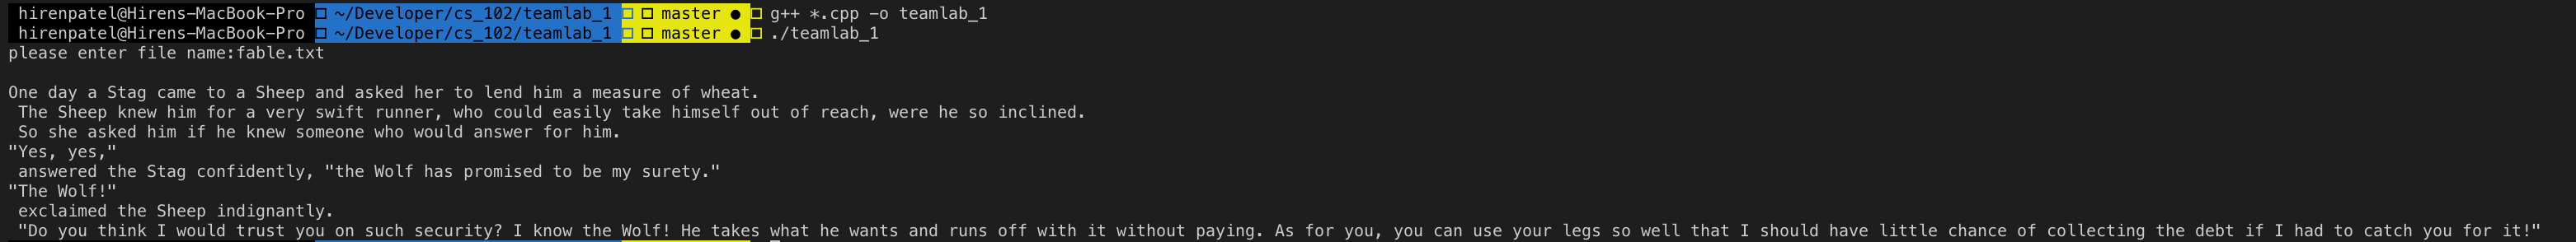
\includegraphics[width=450pt]{img/test1.png}
\begin{verbatim}
This test shows the program compiling than ran. The program asks the user for the file name then displays every sentence
on a new line.
\end{verbatim}
\newpage

\end{document}
